\subsection{Addressing Programs with Conditionals}
    
    Elimination under conditionals can be tricky. 
    For instance, while performing write elimination at the candidate level, we require a write to be agent ordered ahead of it with no intervening read in between (aas stated by the Theorem \ref{WriteElim} and Corollary \ref{CorolWriteElim}).
    In the case of conditionals, the resultant candidates may or may not have such a write depending on whether the conditional is satisfied. 
    While performing read elimination, the read itself can be the conditional check, which then brings the question of why this read would be eliminated by the compiler.
    Note again that we do not assume anything about the optimization being done by the compiler. 
    We only investigate whether eliminating an event is safe to do.  

    We first consider the elimination of write in programs with conditional branches. 
    The following corollary establishes when doing such an elimination is safe: 
    \begin{corollary}
        \label{WriteElimCond}
        Consider a program $P$ and its candidates $C_1, C_2, ... , C_n$ in which events $e$ and $d$ present such that 
        \begin{align*}
            \event{e}{W} \ \wedge \ \event{d}{W} \ \wedge \ \et{e}{uo} \ \wedge \ \reln{e}{ao}{d} \ \wedge \ \Re(e)\!=\!\Re(d).
        \end{align*} 
        Consider the set of corresponding candidates $C'_1, C'_2, ... , C'_n$ after eliminating $e$ and its corresponding program $P'$. If the following two conditions hold
        \begin{gather}
            \forall C_{i \in [1,n]}, \forall k \in C_i \ \text{s.t.} \ \reln{e}{ao}{k} \wedge \reln{k}{ao}{d}, \    
            Reord(e,k). \tag{1} \label{elim:cond_write1}\\   
            \nexists C \ \text{s.t.} \ \event{e}{C} \wedge d \notin C. \tag{2} \label{elim:cond_write2}
        \end{gather}
        then the set of observable behaviors of $P'$ is a subset of that of $P$.
    \end{corollary}

    \begin{proof}
    
        From Condition \ref{elim:cond_write1} we have then for $C_i$
        \begin{align*}
            \forall \ k \ \textit{s.t.} \ 
            \reln{e}{ao}{k} \ \wedge \ \reln{k}{ao}{d} \ . \ 
            Reord(e,k).
        \end{align*}
        The above is Corollary \ref{CorolWriteElim}, thus giving us that the observable behaviors of $C_i'$ is a subset of $C_i$. 
        Hence this condition must hold for all candidates from which we eliminate $e$. 
    
        Suppose Condition \ref{elim:cond_write2} does not hold. 
        Then we have 
        \begin{align*}
            \exists C \ \text{s.t.} \  \event{e}{C} \wedge d \notin C.
        \end{align*}
    
        This would mean, for such a candidate $C$ and its Candidate Executions, by Corollary \ref{CorolWriteElim} the observable behaviors of $C'$ may not be a subset of $C$. 
        Hence observable behaviors of $P'$ may not be a subset of $P$.
        Hence, by contradiction, Condition \ref{elim:cond_write2} must hold\footnotemark. 
    
        \footnotetext{Note that the second condition, by Prop \ref{CondB1} implies $e$ and $d$ cannot be part of different conditional branches.}
        
        Figure~\ref{elim:cond} elicit the cases of conditionals that are allowed by the Condition \ref{elim:cond_write2} below.
        \begin{figure}[H]
            \centering
            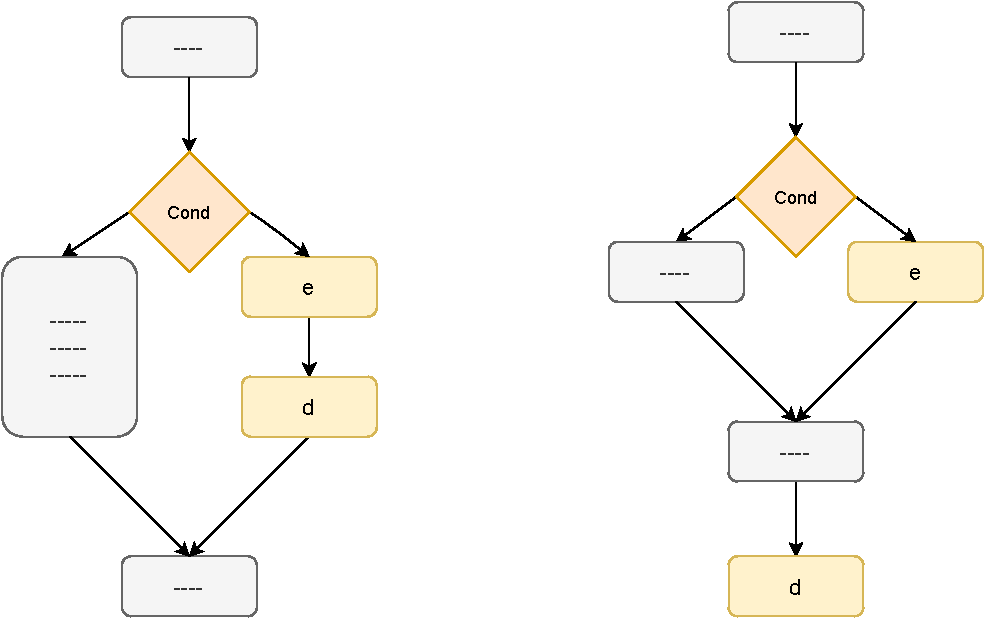
\includegraphics[scale=0.7]{5.Elimination/2.ValidEliminationProgram/Conditionals/ConditionalsCases.pdf}
            \caption{Cases of Conditionals where elimination of $e$ is safe.}
            \label{elim:cond}
        \end{figure}
    
    \end{proof}
    
    As far as read elimination goes, since we only need the information of the read event that is to be eliminated, we do not need additional conditions to hold at the program level when conditionals exist. 
    There is however, one case, in which the read itself is the conditional check. 
    When this is the case, the resultant code after elimination depends on the intention of the compiler, which can be either of the following:
    \begin{itemize}
        \item It could be dead code elimination, wherein both branches of code are eliminated entirely. 
        \item It could be that the conditional check always returns the same value, which makes the branch taken to be the same. 
        \item It could be that the choice of branch does not affect the outcome of the program itself. 
    \end{itemize}
    
    Since we place no assumption on why the compiler would do such elimination, it is not possible to ascertain the target code and their resultant Candidate and Candidate Executions that are intended. 
    Hence we do not address this case and simply state that as long as the read to be eliminated is \textbf{not} a conditional check, it is safe to eliminate under the conditions of Theorem \ref{ReadElim}. 
    